\chapter{Stand der Technik}
\begin{onehalfspace}  
    \label{sec:theorie/standdertechnik}
        In diesem Kapitel wird der Stand der Technik näher beleuchtet. Der Fokus liegt dabei auf den Themen Daten, \ac{KI} und Bias. Zu Beginn wird auf basis der Literatur erläutert, was Daten sind, was Datenqualität bedeutet und worum es sich bei einem Bias handelt. Daraufhin wird näher auf \ac{KI}, das Teilgebiet \ac{ML} und die Ethik in der \ac{KI} eingegangen. Zuletzt werden die Themen in einen gemeinsamgen Kontext gesetzt und der Einfluss eines Bias auf eine \ac{KI} betrachtet und Gegenmaßnahmen untersucht. 
    
    \section{Daten als wertschöpfende Ressource}
    \label{subsec:datenchapter}
    \subsection{Daten}
    \label{subsubsec:daten}
        Dass Daten eine wertvolle Ressource seien, meinte bereits 2006 der britische Mathematiker Clive Humby mit dem berühmten Zitat: \glqq{}Data is the new oil\grqq{}. Hiermit ist gemeint, dass Daten in ihre Rohform nicht sonderlich wertvoll sind, jedoch sobald man beginnt sie zu verarbeitet gewinnen sie an Wert. Lange Zeit waren Daten nur ein Nebenprodukt der Digitalisierung. Daten wurde gesammelt und gespeichert, aber nicht weiter verwendet. Insbesondere durch das rasante Aufkommen des Internet of Things, steigt  die Menge der gesammelten Daten exponentiell an.\cite{Otto2019}
        \begin{figure}[h]
            \centering
            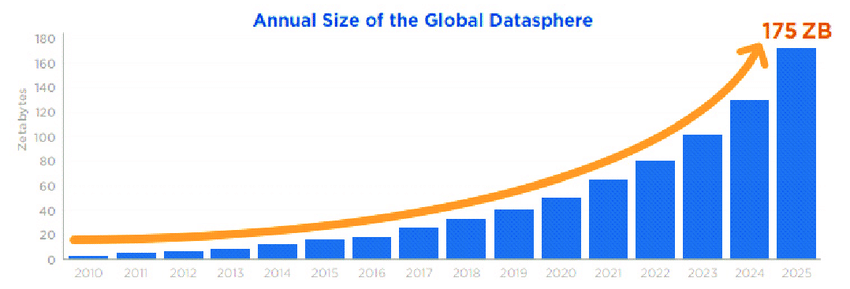
\includegraphics[width = 15cm]{Bilder/Annual_Data_Size.png}
            \caption{Weltweit jährlich anfallende Datenmenge \cite{Reinsel2018}}
            \label{fig:DataSize}
        \end{figure} 
        \\
        Abbildung \ref{fig:DataSize} stammt aus dem Jahr 2018 und verdeutlicht, dass bereits damals erwartet wurde, dass bis im Jahr rund 175 Zetabyte an Daten jährlich genereirt und gesammelt werden. Im Vergleich dazu waren es 2018 gerade einmal 33 Zetabyte an Daten, die weltweit generiert wurden. \cite{Reinsel2018}
        \\
        Der Begriff Daten selbst wird im ISO2382-1 Standard wiefolgt definiert: \glqq{}reinterpretierbare Darstellung von Informationen in einer formalisierten Weise, die für die Kommunikation, Interpretation oder Verarbeitung geeignet ist\grqq{}. \cite{ISO2382} Daten Daten gibt es in unterschiedlicher Form. Meist unterscheidet man zwischen strukturierten und unstrukturierten Daten. 
        \\
        - Daten haben sich von einem Nebenprodukt zu einer wertvollen Ressource entwickelt
        - Daten sind das Öl der zukunft <-- Zitat raussuchen
        - Wir sammeln enorm viel daten --> Big Data --> zig tausende an Zetabyte <-- Quelle suchen
        - Daten ermöglichen neue Geschäftsfelder --> Data Driven Diagnoses, Development, Analytics

    \subsection{Datenqualität}
    \label{subsubsec:datenqualität}
        - Datenqualität spiel eine große Rolle seit wir Daten anfangen analysieren auszuwerten
        - 80 Prozent der Arbeit eines Data Scientist ist das Daten vorverarbeiten aufgrund schlechter Datenqualität
        - Data Quality Management
        - Data Qaulity Richtlinien und Anforderungen
        - Metadaten --> Das wissen über die Daten, was sollten die Daten repräsentieren und tun sie das auch

    \subsection{Bias}
    \label{subsubsec:Bias}
        -   Begriffserklärung: Data Bias vs Bias Verzerrung / Over-/Underfitting (zu viel/zu wenig lernen im ml)\\
        -   Arten von Bias: \\
            -   Bias durch Abwesenheit - Wenn eine Info fehlt, kann das zu Diskriminierung führen. \\
            -   Diskriminierung durch Menschen. \\
        Arten von Bias: Cognitive, Social, Perceptual und Motivational Bias \cite{Parkavi2018}


    \newpage
    \section{Künstliche Intelligenz}
    \label{subsec:KIandML}
    \subsection{Künstliche Intelligenz Allgemein}
    \label{subsubsec:KIAllgemein}
        - Was bildet KI alles ab <-- Grafik B. Otto?
        - KI als Geschäftsfeld 
        - KI und seine potentiale Ausleuchten 
        - Was ist alles KI
        - Wie definiert sich KI


    \subsection{Teilgebiet maschinelles Lernen}
    \label{subsubsec:teilgebietML}
        - Wie funktioniert ML --> Daten die gesammelt werden
        - Bewertete Daten aus der Vergangenheit --> Daten bewerter Jobs <-- Quelle
        - Welche Risiken - over under fitting etc.
        -   Superviced learning --> Data Bias\\
        -   Unsuperviced learning --> nicht zwingend Data Bias\\


    \subsection{Ethik in der künstlichen Intelligenz}
    \label{subsubsec:ethikinderKI}
        - Ethik spielt eine große Rolle in der Gesellschaft
        - EU Setzt sich mit Richtlinien auseinandern
        - Diskriminierung durch KI ist ein fatales Problem
        - Maschinen besitzen keine Moral und Ethisches werteverständnis


    \newpage
    \section{Bias im Zusammenhang mit \ac{KI}}
    \label{subsec:KIundbias}
    \subsection{Diskriminierung durch Bias in Daten}
    \label{subsubsec:diskriminierungdurchverzerrung}
        - Bias in Daten
        - Wie funktioniert Bias in Daten
        - Was ist die Problematik
        - Welche Auswirkungen hat es 
        - Realbeispiele <-- Bewerbungsverfahren

    \subsection{Gegenma{\ss}nahmen}
    \label{subsubsec:gegenmassnahmen}
        - Was kann man dagegen tun?
        - Gibt es möglichkeiten Trainingsdaten künstlich zu erzeugen und so eine neutrale betrachtung zu schaffen
        - Parameter entfernen als Lösung --> Die KI wird aber dadurch schlechter 
        - 

        Wenn der Parameter mit dem Bias entfernt wird, wird das Ergebnis erstmal schlechter. 
        
    \newpage
\end{onehalfspace}